\chapter{Problem and proposed solution} \label{chap:Problem}
The problem at hand is the extraction and inclusion of meta features in the Synthetic Dataset Generator SNOOKER generation process. This generator was initially produced by this study's second supervisor Leonardo Silva Ferreira. Simple generators face the problem of not generating realistic enough data or disclosing private information \citep{disclosure} when using a real dataset as a basis for the generation process.

The generator interface should allow users to select various meta features (explored in Chapter \ref{chap:mf}). Those meta features would be used in the generation process and be present in the final synthetic dataset, allowing for the creation of realistic datasets. 

When picking a generation algorithm, the first step will be to analyse the current generator and check its' methodology. If the current algorithm is not satisfiable enough, a new implementation must be made.

Some evaluation metrics should also be applied, and their results should be made available for the user at the end of the generation process.

\section{Snooker - An Overview}
\label{chap:Snooker}
Before analysing the problem, we should first look at the original generator, trying to understand its internal workings. SNOOKER was developed to bridge the availability gap for Helpdesk's datasets.

This section will present a general overview of the generator, talking about its leading technologies, features and the characteristics of its synthetically generated datasets.

\subsection{Technologies}

SNOOKER was developed using Python\footnote{\href{https://www.python.org/}{python.org}} and several of its libraries. Python is an interpreted, high-level programming language considered the standard for exploratory interactive and computation-driven scientific research \citep{5725235}. The user-generation interaction was handled by creating a graphical user interface (GUI).

The user interface of the generator was developed using PyQt\footnote{\href{https://pypi.org/project/PyQt5/}{pypi.org/project/PyQt5/}}. PyQt is a combination of Python bindings for cross-platform applications that combine all the strengths of Qt and Python \citep{siahaan2019postgresql}. This enables the development of GUI elements using Python Code. A print of the generator's GUI can be found in Figure \ref{fig:general_gui}.

The user can use the standard parameters in the presented interface or personalize the generation inputs as he wishes, fumbling with several interface options. After a short delay, a synthetical tabular dataset is generated after clicking the Generate button.

SNOOKER: A DataSet GeNeratOr fOr HelpdesK SERvices was developed using both technologies. A change in technologies in a study aiming to enhance the original generator would start the process from scratch, which would not be a viable option.

\begin{figure}[t]
  \begin{center}
    \leavevmode
    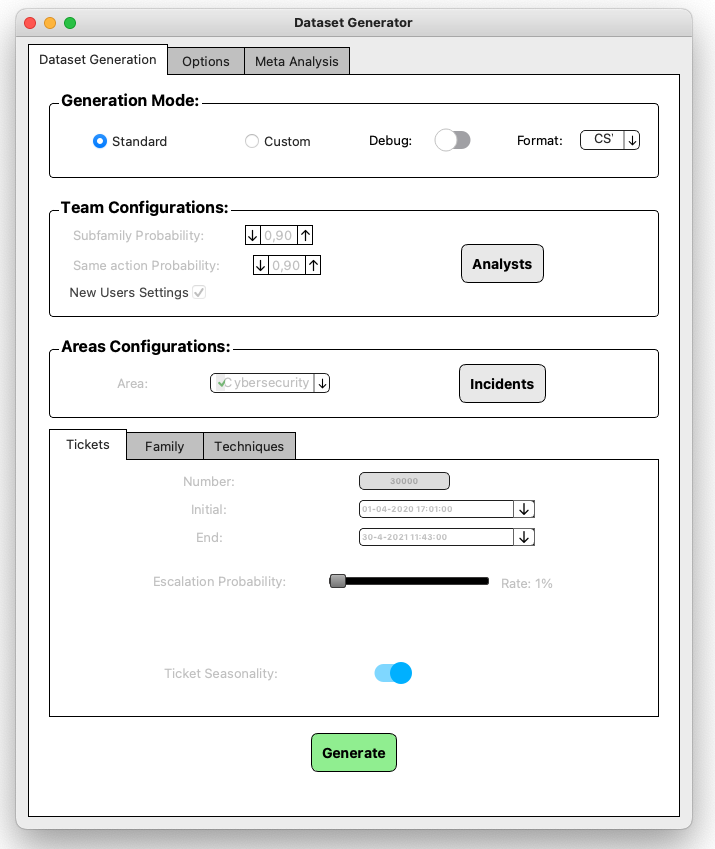
\includegraphics[width=0.6\textwidth]{general_gui.png}
    \caption{SNOOKER's User Interface}
    \label{fig:general_gui}
  \end{center}
\end{figure}

\subsection{Features}
The primary objective of SNOOKER was to enable synthetic helpdesk dataset generation. This dataset would take into account a series of features. The main features included in the generator are ticket management, team management and area management.

Tickets should be able to be customized (quantity, creation time, type, etc.), scheduled, treated (generation of appropriate treatment methods) and replicated if needed. 

The team management module handles the team's statistics (shift management, ticket percentages, etc.) and the singular team member information (general data connected to each member).

Lastly, the area management feature takes care of customizable incidents that might happen in each domain previously described.

It should also be noted that the generator uses as input not only the information provided by the user in the generator's UI but also data from a YAML configuration file.

\subsection{Synthetic Datasets}
SNOOKER's generated datasets contain much information commonly present in helpdesk datasets. While a complete representation of the synthetic dataset is not provided in this section, it can be examined in greater detail in Appendix \ref{ap3:snooker}.
%In this section, we will look at the final output from SNOOKER's generation process, explaining the information in each column of the dataset. The information regarding SNOOKER's outuputed dataset can be found on Appendix \ref{ap3:snooker}. 

\subsection{SNOOKER's generation process}
After receiving input from the previously mentioned configuration file, SNOOKER performs a series of tasks to fully generate each entry on the dataset. 

It starts the process by doing a simple Ticket Creation Task, where all the tickets are generated with simple data, and more complex data is added iteratively. Finally, the ticket family information is inserted in the final phase, where the family distribution over time is considered.

The following module in the generation is the Team Assignment. As its name suggests, this process is responsible for allocating teams and users available for each ticket. Shifts are considered for scheduling ticket-solving tasks by considering the team, work shift, and days not working for each team member.

The User Actions Creation module follows, providing the generator with valid actions (subtechniques) to solve each ticket problem based on its subfamily.

The following module is the Users Assignment. Each ticket is assigned a user and action by using the previously described modules in this process.

The fifth module takes care of Ticket replication tasks. This happens when a ticket is passed to more advanced teams. This event can be triggered when a ticket is created, when a set maximum number of tickets of that subfamily is detected, or when a set distance between the subfamily action and the user action exceeds the maximum distance defined in the interface.

Finally, the last module takes care of generating the Ticket Status. This status can either be 'closed' or 'transferred'. Transferred tickets also need to be replicated and passed to higher teams.

\section{Study Objectives}
Looking back at Chapter \ref{chap:intro} we should take a new look at the questions asked.

What selection of meta features should be calculated from the data in the synthetic dataset? In Chapter \ref{chap:mf}, we extracted several meta features that could be used. The final selection of meta features extracted from our datasets can be found in Chapter \ref{chap:class}.

What generation methods can we use? In Chapter \ref{chap:generation} we analysed a large group of algorithms that can be used to generate synthetic datasets. Of the available options, the one chosen and used later in Chapter \ref{chap:Integration}'s experiments was Conditional distribution. It is also the method used in SNOOKER's generation process.

Can we include specific values of meta features inside the generation process? This is touched on in the final development chapter of this study (Chapter \ref{chap:Integration}), where we study and discuss the possibility of including specific values of meta features inside the generation process.

What new additions can be added to the generator? Allied with the meta feature extraction module, we included a full-fledged meta feature extraction feature into the generator. More information regarding this feature can be seen in Chapter \ref{chap:class}. In Chapter \ref{chap:Conclusion} we also reference some future features that can be added to the application. Besides the inclusion of the new feature no other additions or changes were made to the original generator. 

The development of this study can be considered successful after fully answering the questions and furfilling the objectives presented in this section.

%If possible, the final product should be useful in creating ticket datasets and customisable types of datasets.

\section{Schedule}
Development of the final product went through several steps involving various tasks. A Gantt diagram was created to help with the planning. It can be found in figure \ref{fig:gantt}. 

\begin{figure}[h!]
    \begin{center}
      \leavevmode
      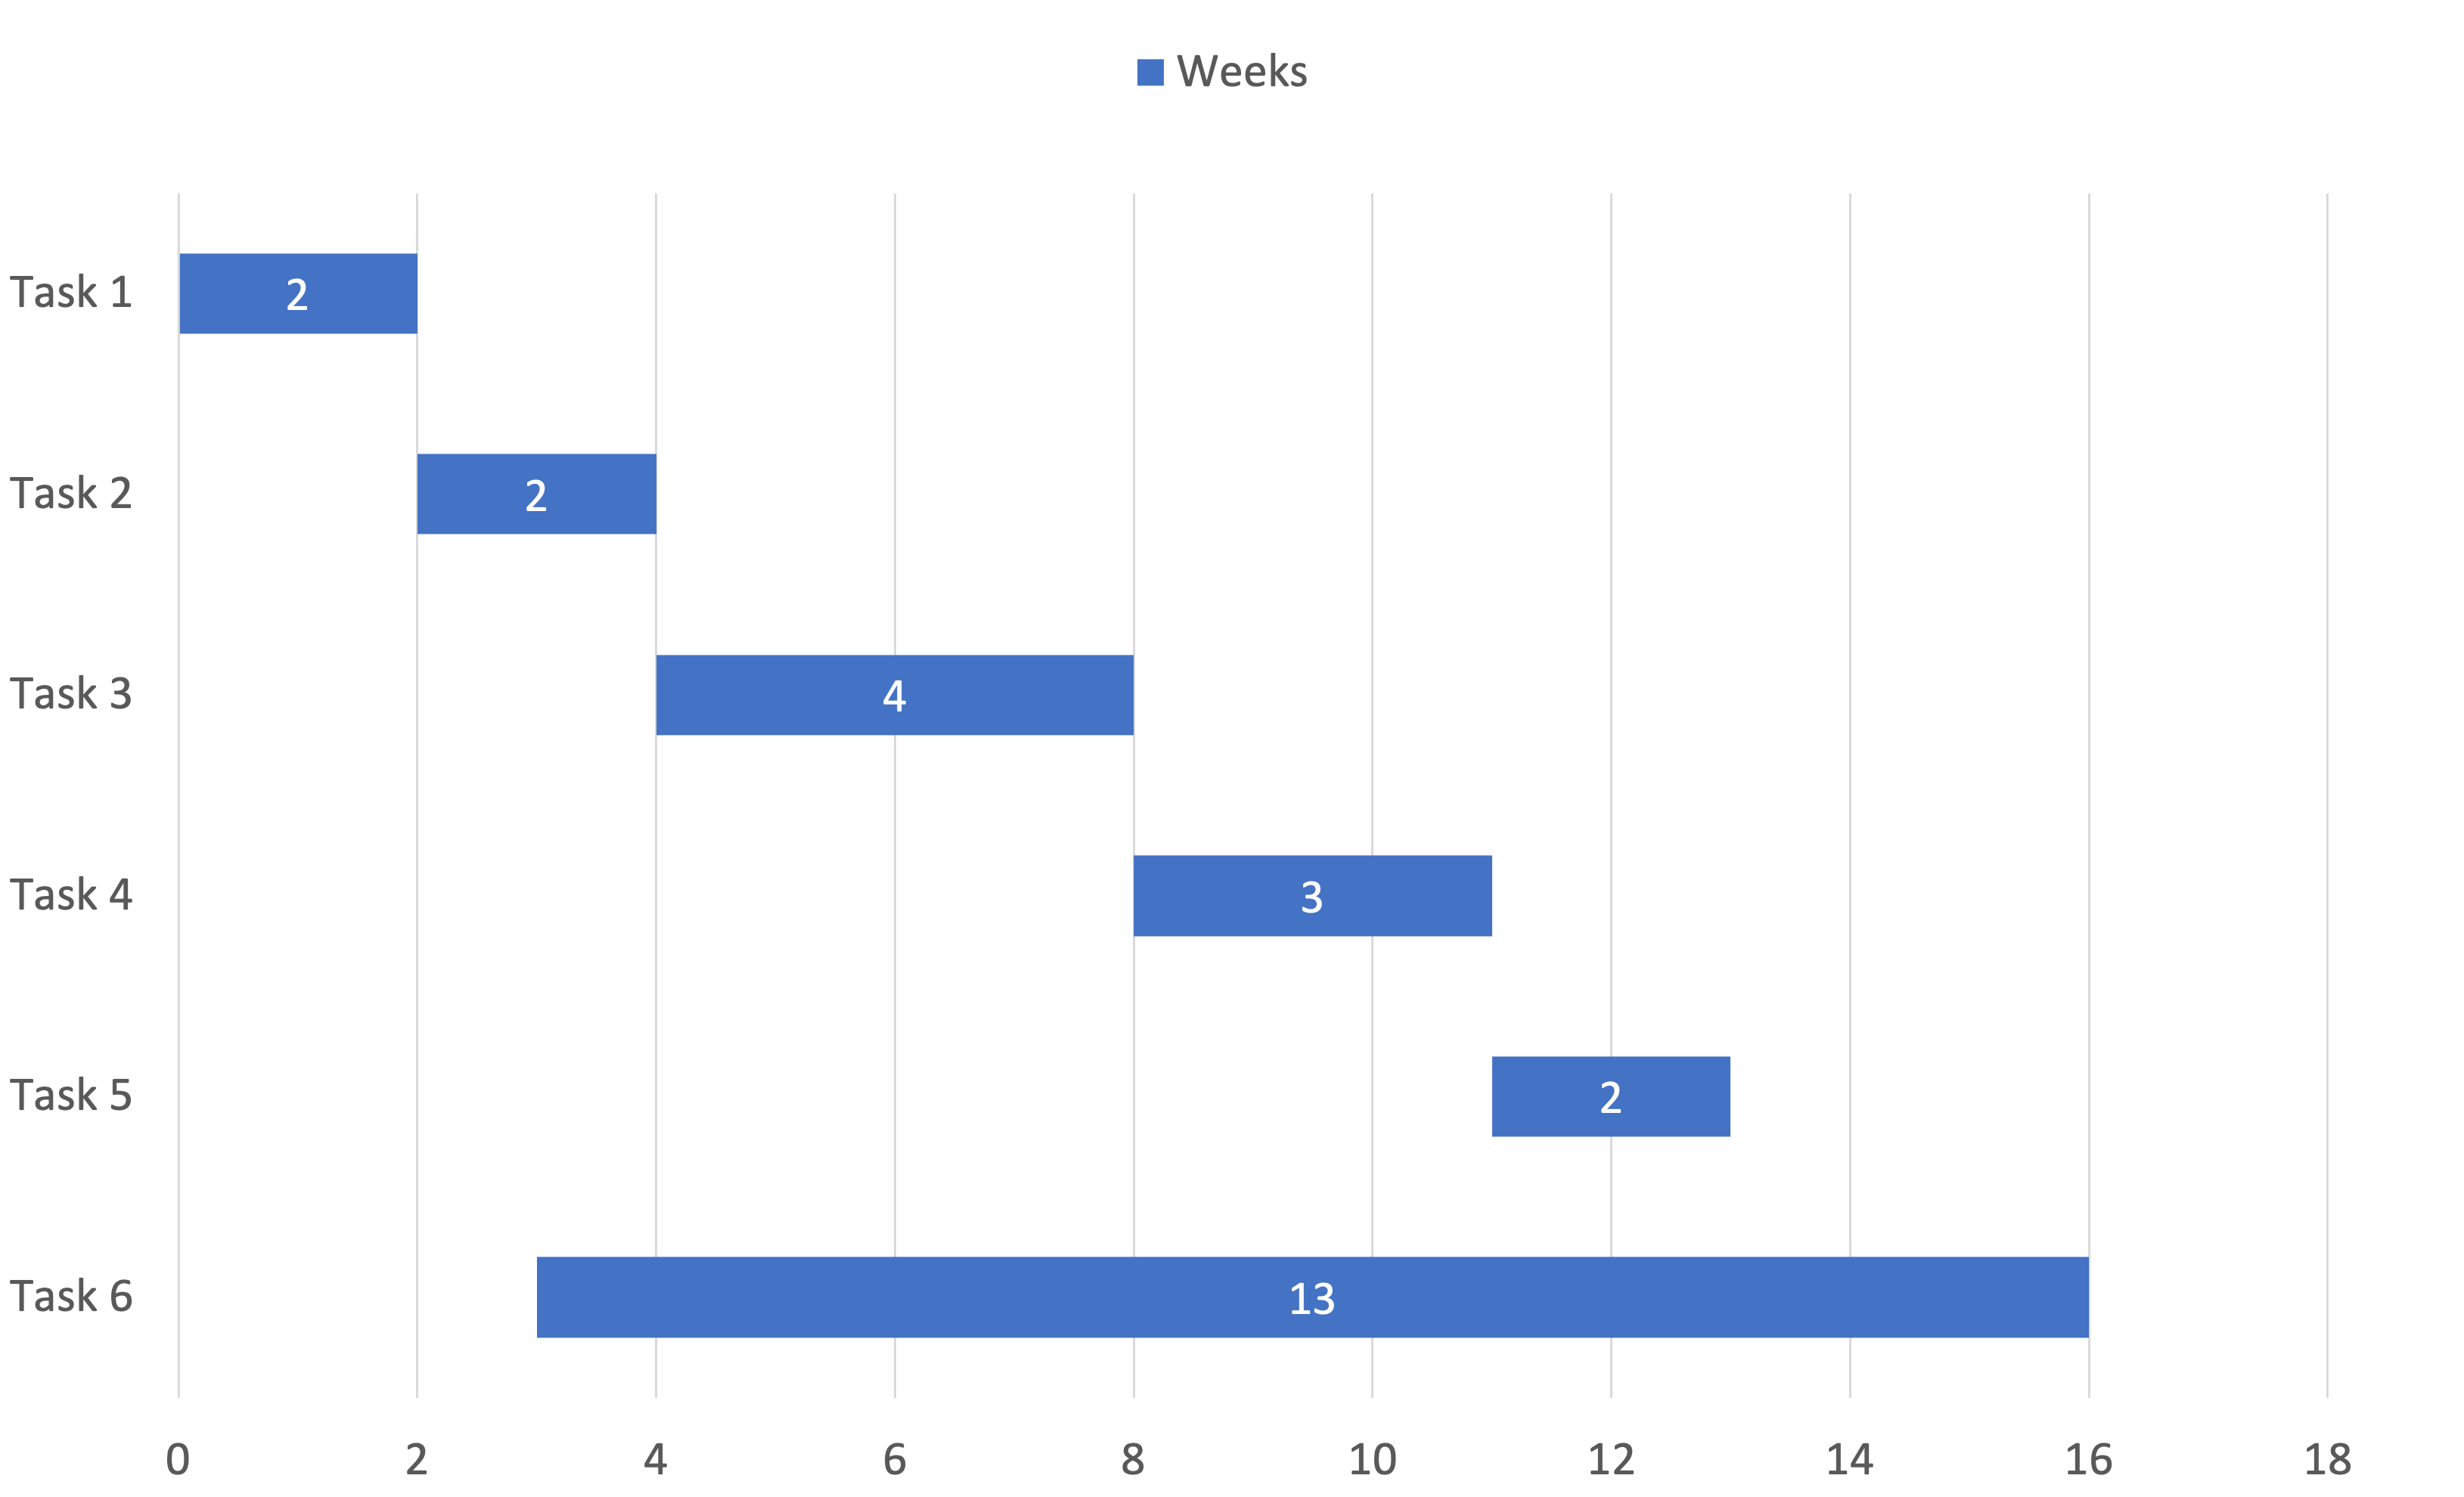
\includegraphics[width=1\textwidth]{gantt.png}
      \caption[Gantt diagram for the developed process]{Gantt diagram for the developed process}
      \label{fig:gantt}
    \end{center}
\end{figure}

Task 1 is the analysis of the current code. Task 2 is the implementation of improvements to the dataset generation process. Task 3 will explore the implementation of some meta feature selection. Task 4 regards quality validation of generated datasets. Task 5 will look at general improvements to the generator, namely in UI/UX. Finally, Task 6 is the writing of the dissertation and scientific paper.


\section{Risk Analysis}
The development of this project faced a series of risks. These risks were hindrances to the development process of the tasks previously depicted. We will now present a series of such potential threats. 

To start, we have to look at time constraints. The task at hand was challenging, and the short amount of time available to complete it made it impossible to deliver every single proposal task at the end.

Hardware limitations also impacted development. As some generation processes and meta feature calculations have high computational costs, an inefficient appliance delays the development, especially during trial-and-error periods. 

Another aspect that impacted development was the lack of know-how when dealing with data analysis and manipulation and the technologies used in the product.

\section{Projected vs Real work}
Ultimately the whole development part ended up not going as far as initially expected. We did not expect so many problems during the development of this project. Problems that ultimately left us still with much open to explore. The author idealised this study as an engineering problem with a core product that would be built upon. But ended up diving more into exploratory subjects, with no concrete answer regarding the inclusion of meta features in generation processes. While we know it is possible to do so, only small results were achieved and not enough to lead to valid proof of concept.

The real work ended up not following the scheduled plan. Analysis tasks took way more time than initially outlined. The quality assurance task became the meta feature extraction feature that took half of the available time to complete. The meta feature implementation (or integration as we now call it) was not fulfilled, being only theoretically explored.

On the other hand, the meta feature extraction tool serves as suitable proof of concept for the problem at hand. While the extraction in high dimensional datasets is still resource-intensive, this tool can perform each extraction task, given enough time.

Left behind were the practical meta feature inclusion module and the inclusion of enhancements to SNOOKER.